\documentclass[11pt,a4paper,titlepage]{article}

\usepackage{pdflscape}
\usepackage[margin=1in]{geometry}
\usepackage{titling}
\usepackage{graphicx}

\graphicspath{ {./Images/} }


\begin{document}
%\title{ \huge Functional Requirements for the SAMBUG}

\begin{titlepage}
    \centering
    \vfill
    {\bfseries\Huge
         Functional Requirements for the SAMBUG project\\
      \hfill\\
         \Large COS301
        \vskip2cm
        \includegraphics[width=6cm]{sambug} \\

    }    
    \vfill
        Abrie van Aardt 13178840\\
		Werner Mostert 13019695\\
		Kele-ab Tessera 13048423\\
		Keagan Thompson 13023782\\
		Michelle Swanepoel 13066294\\
    
    
    \vfill
    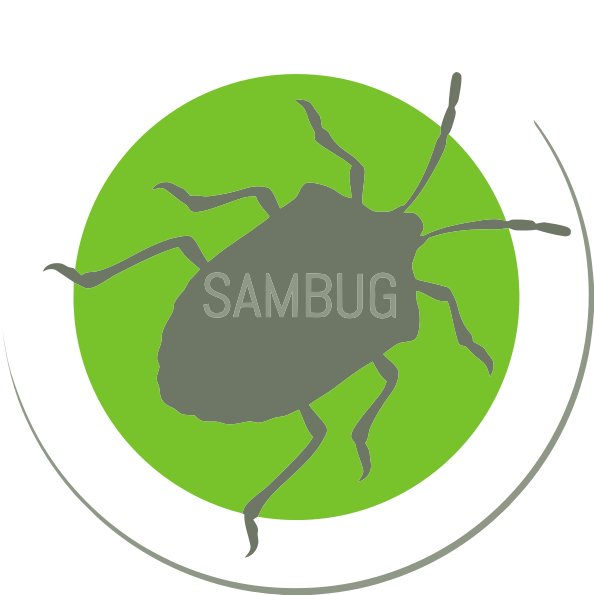
\includegraphics[width=6cm]{logo} \\
    \textbf{May 2015}
    \vfill
\end{titlepage}
	
%\author
%{     
%	Abrie van Aardt 13178840\\
%	Werner Mostert 13019695\\
%	Kele-ab Tessera 13048423\\
%	Keagan Thompson 13023782\\
%	Michelle Swanepoel 13066294\\
%}
    
%\date{\textbf{May 2015}}

%\maketitle

\tableofcontents


% Put all images in images folder - Please use PNG's not Jpegs
% Preferably create separate file for your domain - just like with the use cases
\pagebreak


\section{Background}
South Africa is currently the largest producer of macadamia nuts in the world. One of the main production and quality limiting factors is the incidence of stink bug damage. 
\\Accurate timing of chemical sprays rely on accurate scout data and economic threshold levels of the insect pests in an orchard. However, scouting for these pests has
a major shortfall, namely the accurate identification of pests, despite efforts to train growers and scouts by various means.\\
Area wide control of pests and diseases is a concept that has been considered, but with the lack of scout data from across and within growing regions it is impossible to make such recommendations. \\

\section{Vision}
An innovative approach to handling the management and acquisition of scout data is to develop a smartphone application that is able to identify specific hemipteran species by making use of the built-in camera of the smartphone. This application should ideally be able to make use of the smartphone’s built-in GPS to perform geotagging and uploading information to a central database.

\section{Scope}
\includegraphics[width=\linewidth]{scope}

\section{Architecture requirements}
	\subsection{Access channel requirements}
	\subsection{Quality requirements}
	\subsection{Integration requirements}
	\subsection{Architecture constraints}
\section{Functional Requirements and Application Design}
	\subsection{Domain Model}
	\subsection{BugScouting}
		\subsubsection{Module Scope}
		\subsubsection{Use Cases}
	\subsection{BugIntelligence}
		\subsubsection{Module Scope}
		\subsubsection{Use Cases}
	\subsection{BugSecurity}
		\subsubsection{Module Scope}
		\subsubsection{Use Cases}
	\subsection{BugReporting}
		\subsubsection{Module Scope}
		\subsubsection{Use Cases}

	
		
		
	
\section{Open Issues}


%\pagebreak
%\section{Notifications and Messages Domain}
%  \input{Notifications}

\end{document}